\section{Einführung}\label{sec:introduction}
\IEEEPARstart{S}ysteme zur Spracherkennung finden eine zunehmende Verbreitung und Beliebtheit im alltäglichen Leben. Das Spektrum dieser Anwendungen ist dabei Vielfältig und reicht vom Diktieren von Nachrichten über das Steuern von Geräten bis hin zum Einsatz in Autos. Dabei ist die Qualität der Spracherkennung und die Reaktion des Systems ein entscheidender Faktor, um die Interaktion so natürlich wie möglich zu gestalten \cite{Yu.2014}. Allerdings ergibt sich hier ein Hindernis für mehrsprachige Nutzer. Die natürliche Interaktion wird dadurch behindert, da viele ASR-Systeme den Anwender auf eine voreingestellte Sprache beschränken. In den meisten herkömmlichen Systemen werden Sprachen sowie Dialekte unabhängig voneinander betrachtet. Es wird für jede Sprache ein separates akustisches Modell trainiert [Paper A Real-Time End-to-End Multilingual Speech Recognition Architecture]. Bei weltweit etwa 7000 gesprochenen Sprachen ist es daher nur konsequent, multilinguale Spracherkennungssysteme zu entwickeln \cite{Gary.2018}. Allerdings erfordert ein solches System einen entsprechenden Satz an markierten Trainingsdaten, um wiederkehrende Muster der Sprache zu erkennen. 
Dieser Umstand sorgt für erhebliche Qualitätsunterschiede zwischen den Sprachen, da nicht alle Sprachen über solche Datensätze verfügen. Um die Knappheit der beschrifteten Trainingsdaten zu kompensieren nutzt man den Ansatz der geteilten Hidden Layer [Paper Using Language Adaptive]. Dieser Ansatz stützt sich auf das Zusammenführen aller Daten, um so eine gemeinsame Nutzung der Phoneme zu gewährleisten.  Phoneme stellen dabei eine abstrakte Repräsentation aller Laute einer Sprache dar \citation{Zissman.2001}. Um genaue akustische Modelle für eine große Anzahl von Sprachen effizient und effektiv zu trainieren, um die Kosten, die beim Training dieser Modelle entstehen zu reduzieren und um neue Anwendungsszenarien zu unterstützen, besteht ein wachsendes Interesse an der Entwicklung mehrsprachiger Spracherkennungssysteme \cite{Yu.2014}. 
Zu Beginn erfolgt eine Erläuterung bestimmter Grundlagen, die für das weitere Verständnis der Arbeit wichtig sind. Darauf aufbauend wird erläutert, wie die Identifikation sowie die Erkennung von Sprachen funktioniert. Anschließend werden die Recurrent Neural Networks sowie deren Erweiterung, die Long short-term memory-Netzwerke beschrieben, welche heute im Bereich der multilingalen Spracherkennung verwendet werden. Dabei wird beleuchtet, wie dieses funktioniert und welche Vorteile gegenüber anderen tiefen neuronalen Netzen bestehen. Das Training eines solchen Modells folgt im Anschluss mit einer abschließenden Diskussion bezüglich weiterhin bestehender Probleme und zukünftiger Ansätze.

\section{Verwandte Arbeiten}
Dieses Kapitel stellt exemplarisch wichtige Arbeiten vor, welche mit dem Thema des Artikels in Beziehung stehen. Es gibt viele Forschungsarbeiten auf dem Gebiet der mehrsprachigen und sprachübergreifenden Spracherkennung. Der Artikel konzentriert sich allerdings nur auf diejenigen, die Recurrent Neural Networks bzw. LSTM-Netzwerke verwenden. Der Schwerpunkt dieser Arbeit liegt bei dem Untersuchen dieser Verfahren zur Realisierung entsprechender Systeme sowie die sich hier ergebenden Vorteile gegenüber bisheriger Verfahren. Dabei wird kein detaillierter Vergleich verschiedener Modelle aufgeführt.  
Die Abhandlung lehnt an das Werk Automatic Speech Recognition - A Deep Learning Approach von Dong Yu und Li Deng \cite{Yu.2014} an. Das Buch liefert einen genauen Überblick über die Thematik. Die Grundlagen bezüglich automatischer Spracherkennungssysteme, konventioneller Ansätze und Trainingsverfahren sowie die Architektur mehrsprachiger Systeme werden hier beschrieben.
Ein weiteres für diesen Artikel interessantes Werk ist das Buch Sprachverarbeitung von Beat Pfister und Tobias Kaufmann, in welchem Grundlagen und Methoden der Sprachsynthese und Spracherkennung genau beschrieben werden.  
Des Weiteren gibt    


\section{Hintergrund}
\subsection{Pipeline}
Die Abbildung \ref{fig:pipeline} zeigt die Komponenten, aus dem ein multilinguales Spracherkennungssystem besteht.
Am Anfang steht ein analoges Audiosignal das digitalisiert wird. Aus diesen Daten werden aus kleinen Sequenzen
Feature-Vektoren extrahiert. In Abbildung \ref{fig:pipeline} ist als Beispielausgabe für diesen Teilschritt ein Spektrogramm dargestellt – bei dem die einzelnen Frequenzen bildlich dargestellt werden.
Die Feature-Vektoren müssen so gewählt werden, dass die kleinste effizienteste Menge für die Sprachverarbeitung
entsteht und unnötige Informationen bereits vor dem Decoder herausgefiltert werden.
Die gewonnenen Feature-Vektoren werden als Eingabe für die Sprachidentifikation genutzt. Die Information
über die identifizierte Sprache kombiniert mit den Feature-Vektoren bilden die Eingabe für den Decoder. Der Decoder bildet aus dieser Eingabe,
dem Akkustik-, Sprach- und Lexikalmodell den gesprochenen Text. Die drei Modelle werden von \cite{Tom.2016} wie folgt beschrieben:

\begin{itemize}
    \item \textit{Akkustikmodell.} Die gesprochene Sprache wird abgebildet durch einzelne Phoneme.
    \item \textit{Lexikalmodell.} Alle gültigen Wörter einer Sprache.
    \item \textit{Sprachmodell.} Die Wahrscheinlichkeit für einen syntaktisch und semantisch korrekten Satz.
            Beispielsweise folgt auf das englische Wort \glqq{thank}\grqq{} mit einer sehr hohen Wahrscheinlichkeit das Wort \glqq{you}\grqq{} oder
        \glqq{god}\grqq{}.
\end{itemize}

\begin{figure}[h!]
    \centering
    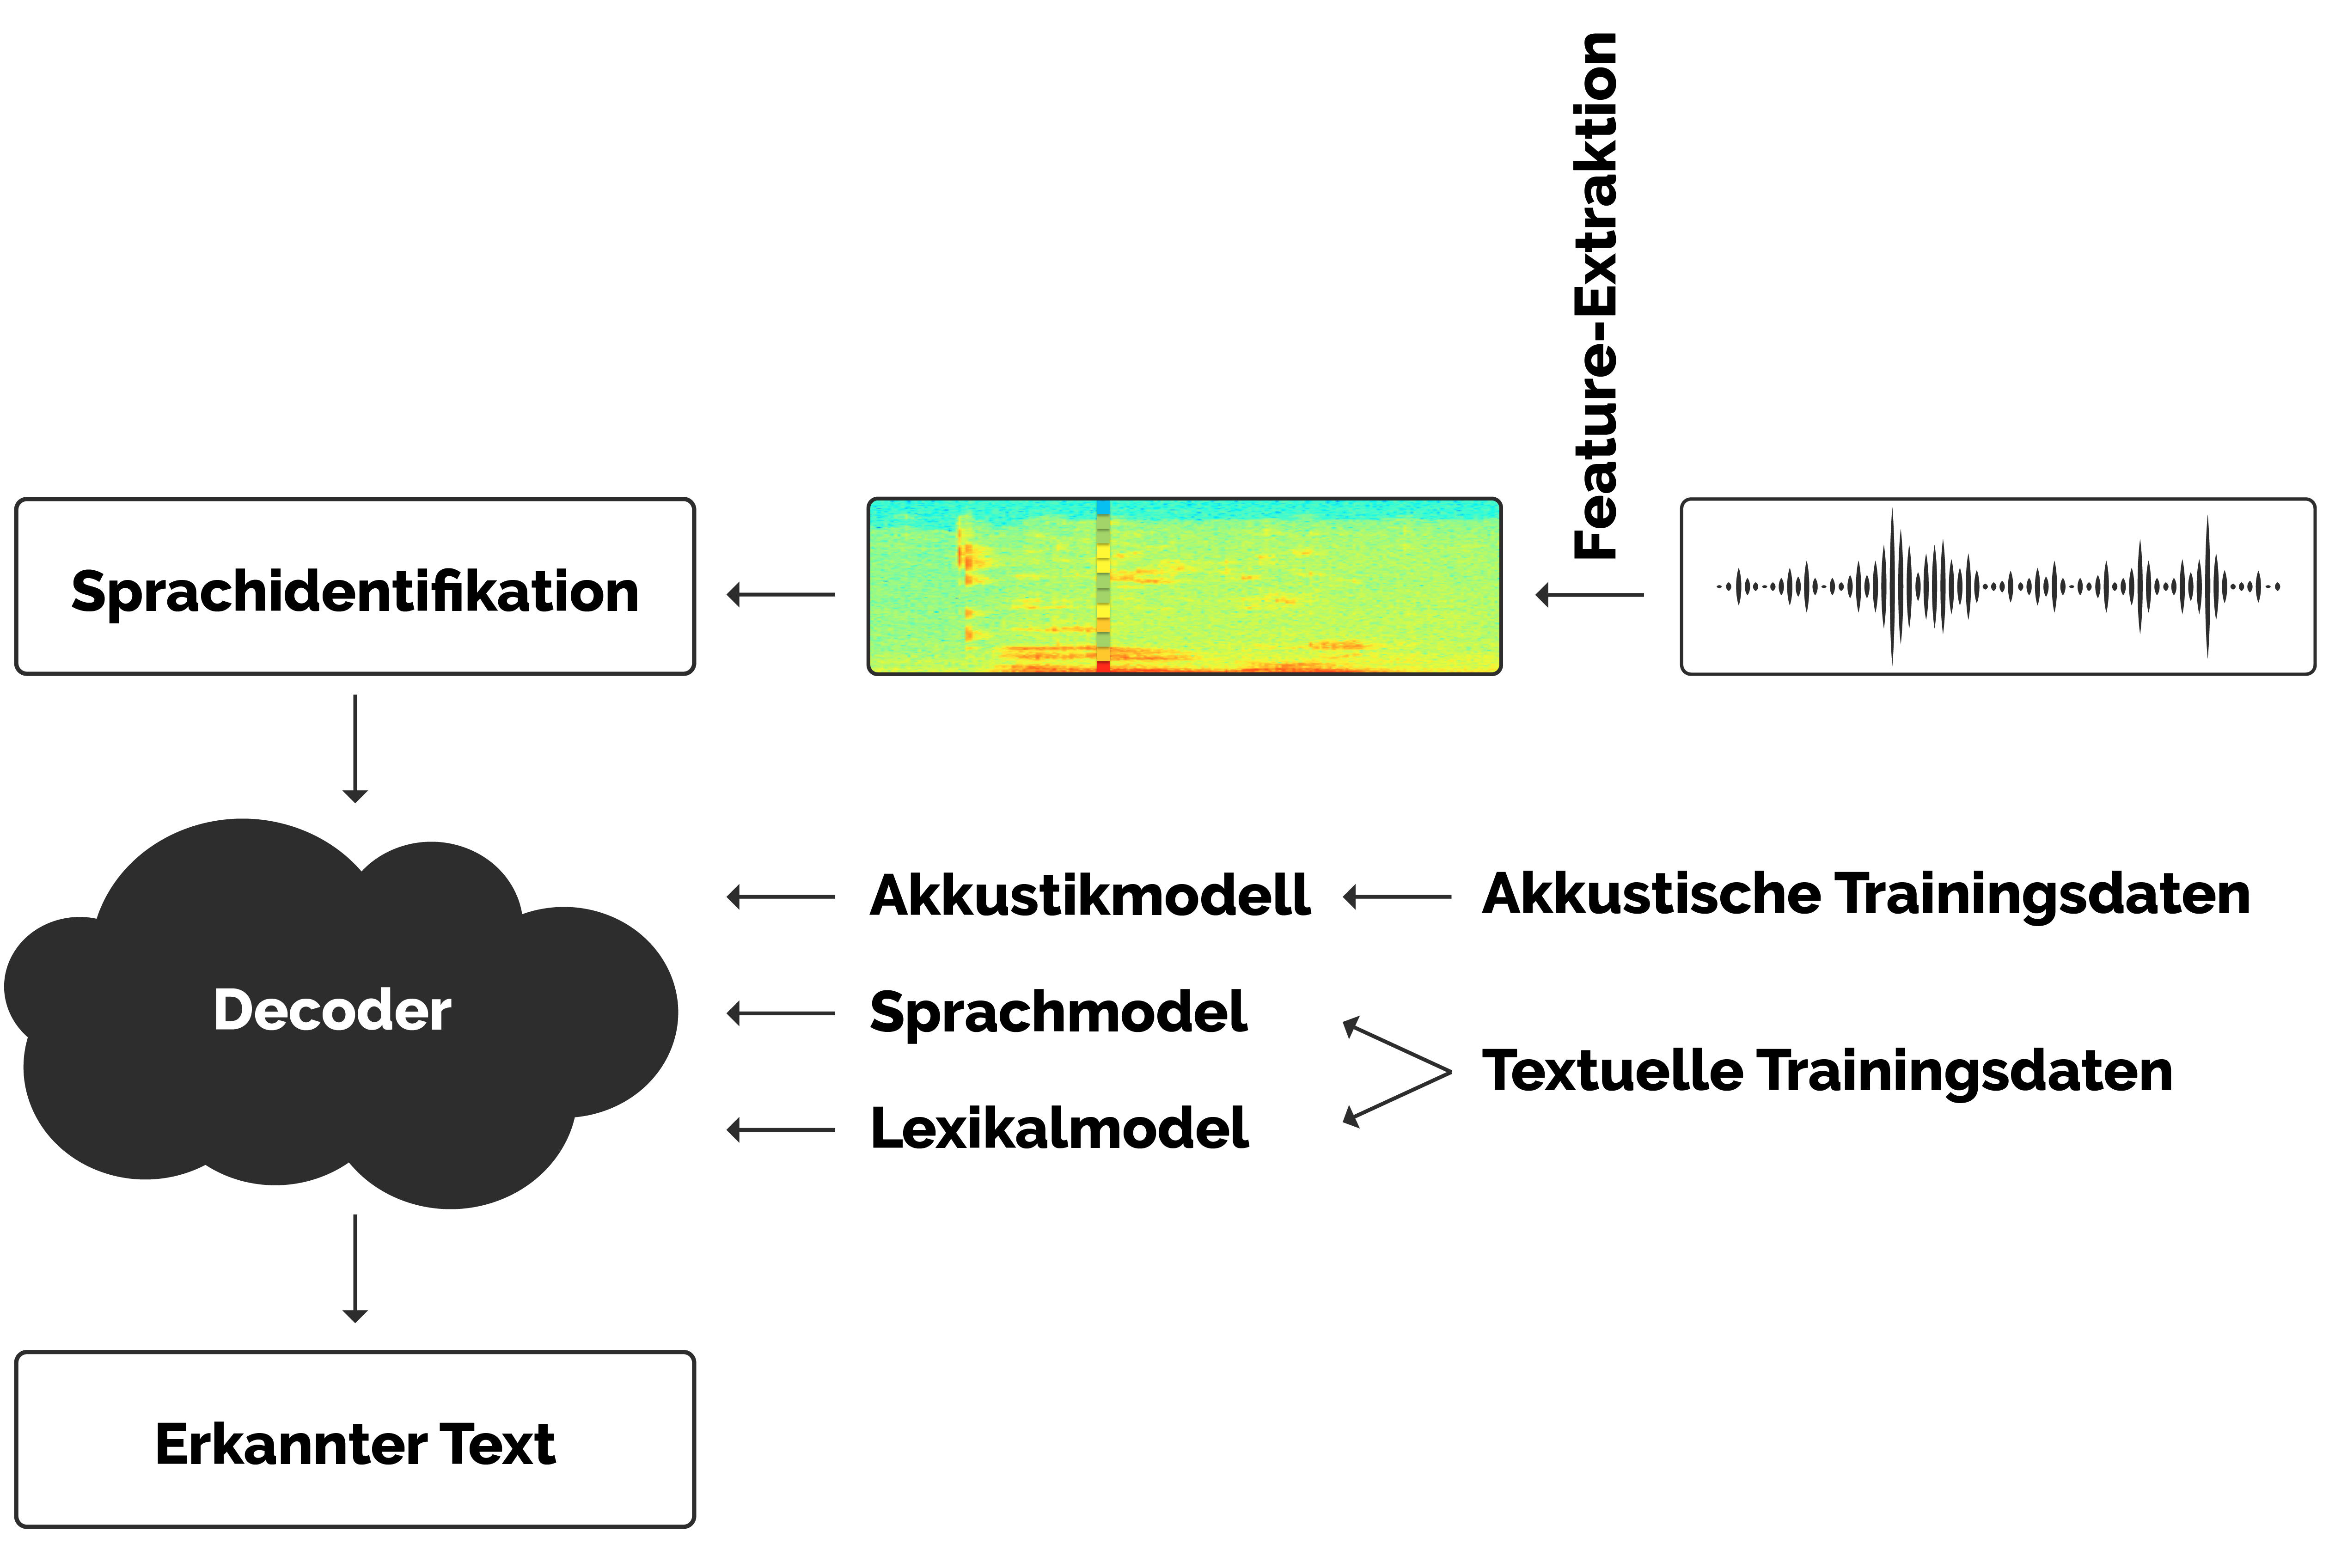
\includegraphics[width=1\linewidth]{images/pipeline}
    \caption{Pipeline eines Spracherkennungssystems (Eigene Darstellung, in Anlehnung an: \cite{Tom.2016}) }%\cite{??}}
    \label{fig:pipeline}
\end{figure}

Die Trainingsdaten für die beschriebenen Modelle werden in die folgenden zwei Gruppen unterteilt \cite{Tom.2016}:

\begin{itemize}
    \item \textit{Akkustische Trainingsdaten.} Diese Daten werden genutzt um das Eingangssignal auf Phoneme abzubilden.
    \item \textit{Textuelle Trainingsdaten.} Bilden Grammatik und semantische Informationen in den Modellen ab.
\end{itemize}